\newpage
\begin{appendices}
%\renewcommand{\thesection}{\Roman{section}\;\;}
\renewcommand{\thesection}{\Alph{section}}


\section{Catalog of symmetric 2D Euclidean instances inside TSPLIB}

The framed box below contains the names of the \textbf{\underline{subset}} of TSPLIB files corresponding to symmetric Euclidean 2D instances. 
The number inside each instance name denotes the number of points e.g. \verb|berlin52.tsp| contains 52 points in $\RR^2$. 
Python has excellent YAML data parsers, and so I've converted the TSPLIB files below into YAML format. 

These converted files files have been stored in the folder


\begin{displayquote}
\color{blue} \Large
\begin{center}
\texttt{./sym-tsp-tsplib/instances/euclidean\_instances\_yaml/}
\end{center}
\end{displayquote}

The original files (i.e the ones with \verb|.tsp| extension) can be found in 

\begin{displayquote}
\begin{center}
\texttt{./sym-tsp-tsplib/instances/tsplib\_symmetric\_tsp\_instances}
\end{center}
\end{displayquote}

\footnotesize
\renewcommand\fbox{\fcolorbox{black}{white}}
\setlength\fboxrule{0.1pt}
\fbox{
  \begin{multicols}{4}
    \begin{itemize}
\item \texttt{a280.tsp}
\item \texttt{berlin52.tsp}
\item \texttt{bier127.tsp}
\item \texttt{brd14051.tsp}
\item \texttt{ch130.tsp}
\item \texttt{ch150.tsp}
\item \texttt{d1291.tsp}
\item \texttt{d15112.tsp}
\item \texttt{d1655.tsp}
\item \texttt{d18512.tsp}
\item \texttt{d198.tsp}
\item \texttt{d2103.tsp}
\item \texttt{d493.tsp}
\item \texttt{d657.tsp}
\item \texttt{eil101.tsp}
\item \texttt{eil51.tsp}
\item \texttt{eil76.tsp}
\item \texttt{fl1400.tsp}
\item \texttt{fl1577.tsp}
\item \texttt{fl3795.tsp}
\item \texttt{fl417.tsp}
\item \texttt{fnl4461.tsp}
\item \texttt{gil262.tsp}
\item \texttt{kroA100.tsp}
\item \texttt{kroA150.tsp}
\item \texttt{kroA200.tsp}
\item \texttt{kroB100.tsp}
\item \texttt{kroB150.tsp}
\item \texttt{kroB200.tsp}
\item \texttt{kroC100.tsp}
\item \texttt{kroD100.tsp}
\item \texttt{kroE100.tsp}
\item \texttt{lin105.tsp}
\item \texttt{lin318.tsp}
\item \texttt{linhp318.tsp}
\item \texttt{nrw1379.tsp}
\item \texttt{p654.tsp}
\item \texttt{pcb1173.tsp}
\item \texttt{pcb3038.tsp}
\item \texttt{pcb442.tsp}
\item \texttt{pr1002.tsp}
\item \texttt{pr107.tsp}
\item \texttt{pr124.tsp}
\item \texttt{pr136.tsp}
\item \texttt{pr144.tsp}
\item \texttt{pr152.tsp}
\item \texttt{pr226.tsp}
\item \texttt{pr2392.tsp}
\item \texttt{pr264.tsp}
\item \texttt{pr299.tsp}
\item \texttt{pr439.tsp}
\item \texttt{pr76.tsp}
\item \texttt{rat195.tsp}
\item \texttt{rat575.tsp}
\item \texttt{rat783.tsp}
\item \texttt{rat99.tsp}
\item \texttt{rd100.tsp}
\item \texttt{rd400.tsp}
\item \texttt{rl11849.tsp}
\item \texttt{rl1304.tsp}
\item \texttt{rl1323.tsp}
\item \texttt{rl1889.tsp}
\item \texttt{rl5915.tsp}
\item \texttt{rl5934.tsp}
\item \texttt{st70.tsp}
\item \texttt{ts225.tsp}
\item \texttt{tsp225.tsp}
\item \texttt{u1060.tsp}
\item \texttt{u1432.tsp}
\item \texttt{u159.tsp}
\item \texttt{u1817.tsp}
\item \texttt{u2152.tsp}
\item \texttt{u2319.tsp}
\item \texttt{u574.tsp}
\item \texttt{u724.tsp}
\item \texttt{usa13509.tsp}
\item \texttt{vm1084.tsp}
\item \texttt{vm1748.tsp}
    \end{itemize}
    \end{multicols}
}
\normalsize

\newpage
\section{Data Tables}

\begin{center}

\begin{longtable}{|l|l|l|}
\caption[Feasible triples for a highly variable Grid]{Feasible triples for 
highly variable Grid, MLMMH.} \label{grid_mlmmh} \\

\hline \multicolumn{1}{|c|}{\textbf{Time (s)}} & \multicolumn{1}{c|}{\textbf{Triple chosen}} & \multicolumn{1}{c|}{\textbf{Other feasible triples}} \\ \hline 
\endfirsthead

\multicolumn{3}{c}%
{{\bfseries \tablename\ \thetable{} -- continued from previous page}} \\
\hline \multicolumn{1}{|c|}{\textbf{Time (s)}} &
\multicolumn{1}{c|}{\textbf{Triple chosen}} &
\multicolumn{1}{c|}{\textbf{Other feasible triples}} \\ \hline 
\endhead

\hline \multicolumn{3}{|r|}{{Continued on next page}} \\ \hline
\endfoot

\hline \hline
\endlastfoot

0 & (1, 11, 13725) & (1, 12, 10980), (1, 13, 8235), (2, 2, 0), (3, 1, 0) \\
2745 & (1, 12, 10980) & (1, 13, 8235), (2, 2, 0), (2, 3, 0), (3, 1, 0) \\
5490 & (1, 12, 13725) & (2, 2, 2745), (2, 3, 0), (3, 1, 0) \\
8235 & (1, 12, 16470) & (1, 13, 13725), (2, 2, 2745), (2, 3, 0), (3, 1, 0) \\
10980 & (1, 12, 16470) & (1, 13, 13725), (2, 2, 2745), (2, 3, 0), (3, 1, 0) \\
13725 & (1, 12, 16470) & (1, 13, 13725), (2, 2, 2745), (2, 3, 0), (3, 1, 0) \\
16470 & (1, 13, 16470) & (2, 2, 2745), (2, 3, 0), (3, 1, 0) \\
19215 & (1, 12, 16470) & (1, 13, 13725), (2, 2, 2745), (2, 3, 0), (3, 1, 0) \\
21960 & (1, 12, 16470) & (1, 13, 13725), (2, 2, 2745), (2, 3, 0), (3, 1, 0) \\
24705 & (1, 12, 16470) & (1, 13, 13725), (2, 2, 2745), (2, 3, 0), (3, 1, 0) \\
27450 & (1, 12, 16470) & (1, 13, 13725), (2, 2, 2745), (2, 3, 0), (3, 1, 0) \\
30195 & (2, 2, 2745) & (2, 3, 0), (3, 1, 0) \\
32940 & (1, 13, 16470) & (2, 2, 2745), (2, 3, 0), (3, 1, 0) \\
35685 & (1, 13, 13725) & (2, 2, 2745), (2, 3, 0), (3, 1, 0) \\
38430 & (1, 13, 10980) & (2, 2, 2745), (2, 3, 0), (3, 1, 0) \\
41175 & (1, 12, 13725) & (1, 13, 10980), (2, 2, 2745), (2, 3, 0), (3, 1, 0) \\
43920 & (1, 13, 10980) & (2, 2, 2745), (2, 3, 0), (3, 1, 0) \\
46665 & (2, 2, 2745) & (2, 3, 0), (3, 1, 0) \\
49410 & (2, 2, 2745) & (2, 3, 0), (3, 1, 0) \\
52155 & (1, 12, 16470) & (1, 13, 13725), (2, 2, 2745), (2, 3, 0), (3, 1, 0) \\
54900 & (1, 13, 13725) & (2, 2, 2745), (2, 3, 0), (3, 1, 0) \\
57645 & (1, 13, 13725) & (2, 2, 2745), (2, 3, 0), (3, 1, 0) \\
60390 & (1, 12, 13725) & (2, 2, 2745), (2, 3, 0), (3, 1, 0) \\
63135 & (1, 13, 16470) & (2, 2, 2745), (2, 3, 0), (3, 1, 0) \\
65880 & (1, 13, 16470) & (2, 2, 2745), (2, 3, 0), (3, 1, 0) \\
68625 & (2, 2, 2745) & (2, 3, 0), (3, 1, 0) \\
71370 & (1, 13, 13725) & (2, 2, 2745), (2, 3, 0), (3, 1, 0) \\
74115 & (1, 12, 13725) & (2, 2, 2745), (2, 3, 0), (3, 1, 0) \\
76860 & (1, 13, 13725) & (2, 2, 2745), (2, 3, 0), (3, 1, 0) \\
79605 & (1, 13, 13725) & (2, 2, 2745), (2, 3, 0), (3, 1, 0) \\
82350 & (1, 12, 13725) & (2, 2, 2745), (2, 3, 0), (3, 1, 0) \\
85095 & (1, 12, 13725) & (1, 13, 10980), (2, 2, 2745), (2, 3, 0), (3, 1, 0) \\
87840 & (1, 13, 16470) & (2, 2, 2745), (2, 3, 0), (3, 1, 0) \\
90585 & (1, 13, 16470) & (2, 2, 2745), (2, 3, 0), (3, 1, 0) \\
93330 & (1, 13, 13725) & (2, 2, 2745), (2, 3, 0), (3, 1, 0) \\
96075 & (1, 13, 16470) & (2, 2, 2745), (2, 3, 0), (3, 1, 0) \\
98820 & (1, 13, 16470) & (2, 2, 2745), (2, 3, 0), (3, 1, 0) \\
101565 & (1, 13, 13725) & (2, 2, 2745), (2, 3, 0), (3, 1, 0) \\
104310 & (1, 13, 16470) & (2, 2, 2745), (2, 3, 0), (3, 1, 0) \\
107055 & (1, 13, 13725) & (2, 2, 2745), (2, 3, 0), (3, 1, 0) \\
109800 & (1, 13, 13725) & (2, 2, 2745), (2, 3, 0), (3, 1, 0) \\
112545 & (1, 12, 16470) & (1, 13, 13725), (2, 2, 2745), (2, 3, 0), (3, 1, 0) \\
115290 & (1, 13, 16470) & (2, 2, 2745), (2, 3, 0), (3, 1, 0) \\
118035 & (1, 13, 13725) & (2, 2, 2745), (2, 3, 0), (3, 1, 0) \\
120780 & (1, 13, 16470) & (2, 2, 2745), (2, 3, 0), (3, 1, 0) \\
123525 & (1, 13, 13725) & (2, 2, 2745), (2, 3, 0), (3, 1, 0) \\
126270 & (1, 12, 16470) & (1, 13, 13725), (2, 2, 2745), (2, 3, 0), (3, 1, 0) \\
129015 & (2, 2, 2745) & (2, 3, 0), (3, 1, 0) \\
131760 & (2, 2, 2745) & (2, 3, 0), (3, 1, 0) \\
134505 & (1, 13, 16470) & (2, 2, 2745), (2, 3, 0), (3, 1, 0) \\
137250 & (1, 13, 13725) & (2, 2, 2745), (2, 3, 0), (3, 1, 0) \\
139995 & (2, 2, 2745) & (2, 3, 0), (3, 1, 0) \\
142740 & (2, 2, 2745) & (2, 3, 0), (3, 1, 0) \\
145485 & (1, 12, 16470) & (1, 13, 13725), (2, 2, 2745), (2, 3, 0), (3, 1, 0) \\
148230 & (2, 2, 2745) & (2, 3, 0), (3, 1, 0) \\
150975 & (1, 13, 16470) & (2, 2, 2745), (2, 3, 0), (3, 1, 0) \\
153720 & (1, 12, 13725) & (2, 2, 2745), (2, 3, 0), (3, 1, 0) \\
156465 & (1, 13, 13725) & (2, 2, 2745), (2, 3, 0), (3, 1, 0) \\
159210 & (1, 13, 13725) & (2, 2, 2745), (2, 3, 0), (3, 1, 0) \\
161955 & (1, 13, 16470) & (2, 2, 2745), (2, 3, 0), (3, 1, 0) \\
164700 & (1, 13, 13725) & (2, 2, 2745), (2, 3, 0), (3, 1, 0) \\
\end{longtable}
\end{center}
	 % Separate data file for storing and loading tables.

\newpage
\section{Installing and running the Code}
\label{sec:install}

The program can be downloaded from Github: \url{https://github.com/gtelang/tspnng}. Alternatively
open a terminal and run the command, \texttt{git clone https://github.com/gtelang/tspnng.git}

The only other prerequisites for running the code, are the 
\href{https://www.anaconda.com/products/individual}{Anaconda} distribution of Python 3 
and a couple of other packages.  To check if the Python executable is in your path (and that it is Python 3.7\texttt{+}) 
run the command \verb|python --version|. If it succeeds, you have installed Anaconda! 

The additional packages required can be installed by: 

\begin{quote}
\color{blue}
\texttt{pip install colorama prettytable tsp} \footnote{If you don't have superuser access during installation, add the flag \texttt{\color{red} \texttt{-{}-}user} at the end}   \\
\texttt{git clone https://github.com/jvkersch/pyconcorde} \\
\texttt{cd pyconcorde}\\
\texttt{pip install -e .}
\end{quote}

%#If the installation of \texttt{pyconcorde} fails, that's okay!; the code will switch to the much slower Python based TSP solver that also computes optimal solutions. 
%This slower package can compute tours of size upto 30 to 40 in a few seconds; lareger point-clouds will take more than a couple of minutes.  

To run the program, \texttt{cd} into the code's top-level folder, then type \footnote{On Windows replace, the forward slash `/` by `\textbackslash`}
any one of: 

\begin{itemize}
\item \verb|python src/main.py --interactive|
\item \verb|python src/main.py --batchtest|
\item \verb|python src/main.py --file <points.yaml>|
\end{itemize}



\subsection{Interactive Mode}


In this mode, one can mouse-in points onto a canvas (with double-clicks), run various network algorithms 
and render them onto a GUI canvas. \textit{\footnotesize By the way, make sure the terminal is visible at all times during your 
interaction with the canvas, as it will often ask for input via prompts or display output information.}


\begin{description}
\item[Entering points with mouse clicks] After you  mouse in your input points, press \colredt{i}; that will open a prompt at the terminal, asking which 
network do  you want computed on those points. Enter the code inside the brackets \colredt{(...)} 

\item[Generating large random point-sets on the canvas] If you \textit{don't} want to mouse-in points, and just need random points plastered uniformly across the canvas, 
press \colredt{u}, and then type into the terminal the number of points. Ditto for non-uniformly distributed points: 
only that you must press \colredt{n}. 

  \textit{Note that after generating these points, you can continue mousing in additional points as part of the input. Useful 
  if you want, say, an example with more or less uniform randomly generated points, except for a few small tight clusters here and there. }

\item[Computing TSP directly] \footnote{This is an option meant more for convenience than anything really; might be useful for trying to detect counter-examples}.   
To directly compute the TSP cycle on the points (without needing to go through the prompts of the previous step) just press \colredt{t}. 

\item[Canvas should be active during keypresses] Note that when you press, any of the keys above, your matplotlib canvas \textit{must} be an active window 
\footnote{Single click or tap the window title bar with the mouse to make the canvas active.} . Only \textit{then} 
does matplotlib detect the key presses (i.e. execute the appropriate call-back function).  

\item[Modifying input] If you want to insert another point onto the existing point-set, just double-click at that position on the canvas. 
The computed networks are wiped clean off the canvas, and you can again compoute the appropriate networks again as above. 

\item[Wiping the canvas clean] If you want the screen and the internal state wiped clean completely --- say, to begin tinkering with a fresh set of points --- press \colredt{c}. 
\end{description}

\vspace{2cm}


\begin{mdframed}
{\footnotesize \it
P.S: You may see a warning --- as I do --- in the terminal during key-presses:

\begin{quote}
\color{blue}
\verb|CoreApplication::exec: The event loop is already running|
\end{quote}

{\color{red} Please ignore it!} It doesn't affect any of the results. Something in the
the internals of Matplotlib using Qt triggers that message. \shrug. 
If you have any trouble --- or detect a bug! ---  we can hash things out on Slack, Github or email.
}
}
\end{mdframed}
\newpage
\section{Laundry-list of Questions/Variants/Conjectures}
 \label{sec:questions}


\begin{description}
\item[\color{red} HAMILTONICITY STRUCTURE] We know that the Delaunay Triangulation of a set of points need not be Hamiltonian. In fact \textit{detecting}
      Hamiltonicity of a Delaunay Triangulation is famously $NP$-complete \cite{dillencourt1996finding} 

      Two useful facts before we proceed: 

     \begin{description}
       \item[Folklore] The cube of any connected graph is Hamiltonian. 
             \footnote{It is sufficient to prove this fact for any tree, and then use it on the spanning tree of the given graph}. 
       \item[Fleischner's theorem  \cite{georgakopoulos2009short}] The square of 
             any 2-vertex connected graph is Hamiltonian. 
          \footnote{This last theorem certainly applies to Delaunay triangulations of general point-sets. By the square of a delaunay triangulation, I mean to say: throw away the edge weights and consider the square of the underlying unweighted graph. Once the new edges are added, consider them weighted with the natural euclidean distance between their endpoints}
     \end{description}

     And so the following questions are natural:

     \begin{itemize}
      \item Based on the experiments results shown in this report, can we 
            claim  $TSP \subseteq DT^{k}$ or $TSP \subseteq MST^{k}$ in $\RR^2$ 
           for a \textit{small} constant $k$? I'd wager $k=2,3$ or, at worst, some 
           very slowly growing function of $n$ \footnote{$\log (n)$ maybe?}

      \item For $G=MST^3$, how good is the any (or the shortest??) Hamilton cycle through $G$
            in approximating the TSP? \footnote{This is a cute vertex analog of the standard edge-doubling based 2-OPT heuristic, but is detecting such a cycle for a small MST power polytime? I'd bet yes. Probably the FPT experts have something to say on this topic.}  
            Surely, this must be known, right?  For the arrangement of $n$ points at the roots of unity suggests that the 
            approximation could be as bad as 3. 

       \item What is the likelihood of $MST^2$ of $n$ points $\in \RR^2$ in general position being Hamltonian? 
             Any characterization of such point-sets? 

       \item Given a set of points in $\RR^2$, does *ANY* 
             (weakly/strongly) simple polygon and *ANY* triangulation on those 
             points have an edge in common? This is surely not true, right?!
       
             \large{\textbf{UPDATE}}: Yeah this isn't true.  \autoref{fig:hugo-example} is a nice counter-example due to Hugo. 
             \begin{figure}[H]
             \centering
             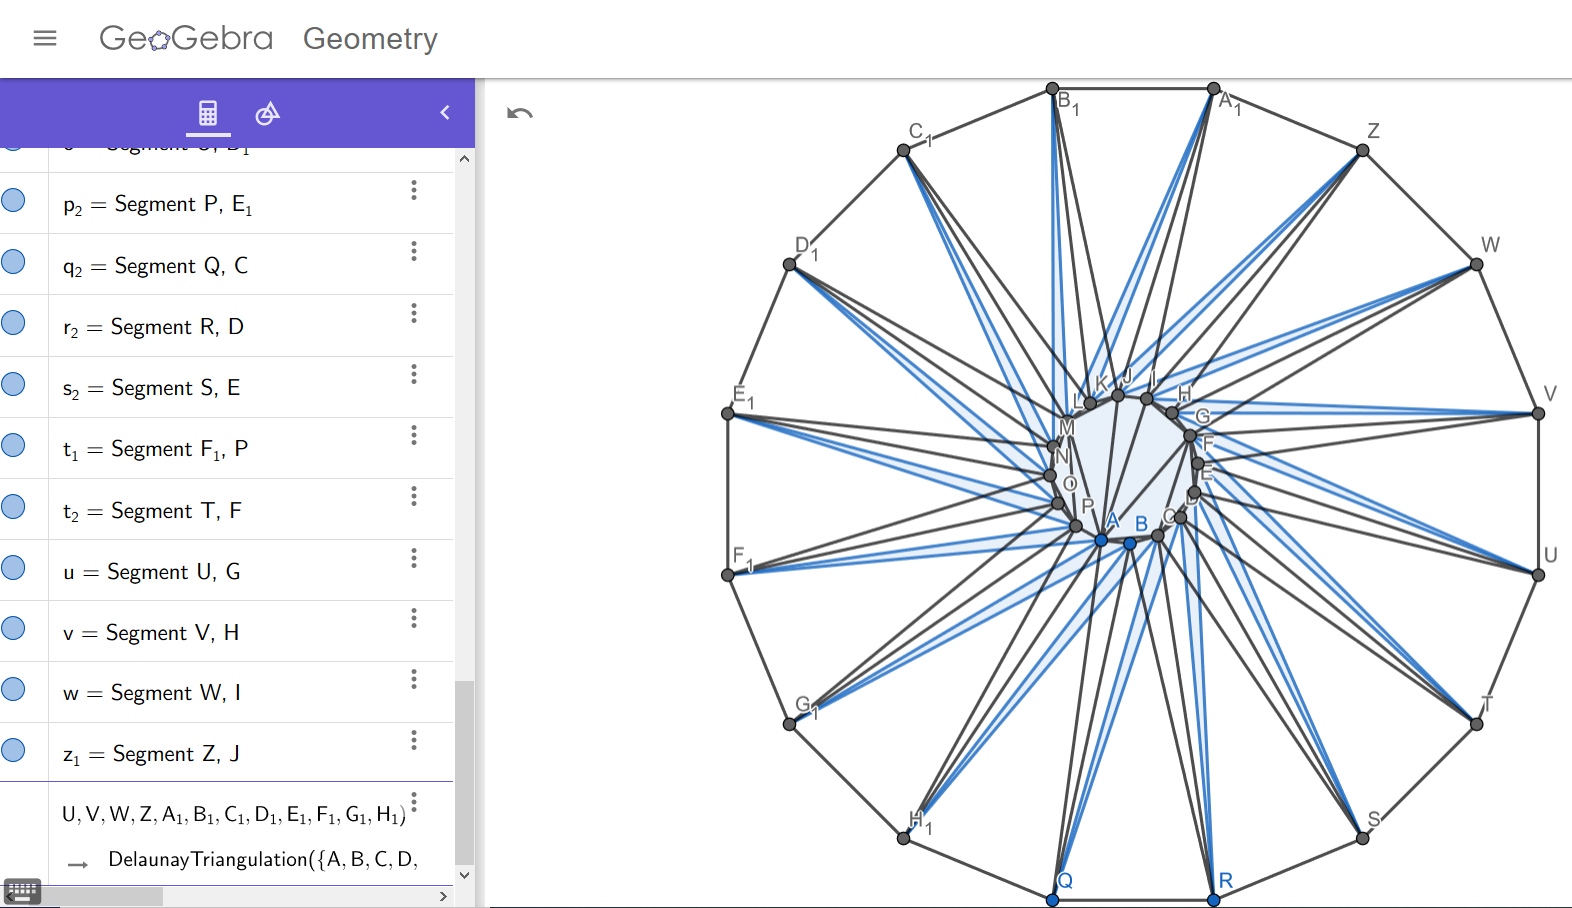
\includegraphics[width=8cm]{miscimages/hugo-example.png}
             \caption{\label{fig:hugo-example} A simple polygon with edges in the complement of the graph of a point set's triangulation}
             \end{figure}

             \textit{Monkey wrench \ala Joe's Universal Guarding Problem:}
             given a set of points $P$ in general position, might there exist a ``universal'' triangulation of $P$ that shares some edge with  
             \textit{any} simple polygon on $P$? Maybe Hugo's counter-example of \autoref{fig:hugo-example} still holds? Qian's beautiful UGP 
                           counterexample from her paper may also be of some relevance. 
                           If this is not true for all point-sets, is detecting this property $NP$-hard? Check if some of the gadgets from 
                           Demaine et al's hardness proof of the pulley problem are applicable here: they basically showed that detecting
                           whether a set of mutually disjoint disks(not necessarily of the same radii) admit a ``pulleygon'' --- excuse the pun! --- is \nph. 
      \end{itemize}
 

\item[\color{red} TSP $\longsquiggly$ DELAUNAY] 

\begin{itemize}
   \item  (Worst idea in history??) Suppose by some magic black box (Concorde! \Winkey) one has obtained the TSP tour through $n$ points.  
          Can we then compute the Delaunay Triangulation (or MST. Recall $MST \subseteq DT$  ) of the point-set 
          in $O(n)$ time? It certainly seems so going by the high number of edges in the TSP common to the Delaunay 
          and MST as suggested by the tests in this writeup. Surely the $TSP \rarr MST$ question in $O(n)$ time has been studied?
          Maybe the Okabe book on Voronoi etc. has something on this? 
          
          
          It's, of course, utter baloney attempting to compute good triangulations or MSTs like this in practice but 
          why should  that \textit{that} stop a computer scientist speculating from the comfort of his/her armchair?


          In some vague sense might be related to the question of \textit{detecting}
          if a triangulation is Delaunay is linear time (check with joe, if this problem is trivial/open/known. I mean 
          detecting if a list is sorted is trivially doable in $O(n)$ as opposed to sorting which takes 
          $\Omega(n \lg n)$ in comparsion model. Are there lower bounds in other models (streaming, online etc.) 
          for Delaunay tri detection? Check with Joe, Mayank others. 
          
          This reminescent of Melkman (i.e. simple poly chain $\rarr$ convex hull in $O(n)$). Samir Khuller also had work (SODA 1992, iirc) 
          in which he was able to compute a $O(1)$ (1.25, was it?) approximations to low-weight spanning trees of max degree 3 on point-sets in $\RR^2$, 
          from a \textit{given} MST in linear time. His paper hinged overall on a very simple but beautiful generalization of the $\Delta$ inequality 
          \footnote{which bounded the perimeter of a triangle in terms of the sums of the distances of a point $X$ to the points of that triangle. When we set $X$ to any of the vertices of the triangle, we recover the standard $\Delta$ inequality. I forget the exact coefficients of that cited linear inequality, remember some $3 \sqrt{3}$ and a 4 in there.}
          Might that be exploitable? Check! 

          Joe mentioned last week there is some nice work by Melhorn et al, on the reconstructibility properties of the TSP back from SOCG 1988(1989?) ;  Also
          Amenta (Crust algorithm) and Dey's works on reconstruction. Maybe we can connect these two lines in some hand-wavy way?  

   \item  Is the Min Weight (MW), or even better, the Min-Angle Maximizing (MAM) Triangulation of the TSP and its external pockets close 
          to being Delaunay in some sense\footnote{e.g. how good is the maximum value of the minimum angle in a triangle over all triangles different from OPT}?  
          Note that both MW and MAM triangulations of simple polygons can be computed by D.P. Should be fun to try this out experimentally. See also Sandor's 
          ALENEX paper from 2015 where he did something about computing "bad" triangulations (iirc he wanted to minimize maximum angle i.e. make triangle skinny), 
          Maybe we could compare against the triangulations obtained from his code, just to see how bad the TSP $\rarr$ Delaunay heuristic is compared 
          to the ``bad end'' of the spectrum? 

\end{itemize}  

\item[\color{red} SHOWING \cite{lin1973effective} HAS A CERTAIN FRACTION OF DELAUNAY/NNG EDGES] 
     Here we try to show that the output of the Lin Kernighan heuristic (rather than the optimal TSP) on any set of points has the postulated properties. In many practical 
     cases, the LK heuristic is optimal, so this might be a cut-price (but interesting) substitute of the original question, especially for lower bounds. 
     The LK paper has also documents some nice local properties of the exchanges.
     \newpage 

     \autoref{fig:linkernighan} is a screenshot from the opening pages:
 
\renewcommand\fbox{\fcolorbox{black}{white}}
\setlength\fboxrule{0.1pt}
   
\begin{figure}[H]
  \centering
  \fbox{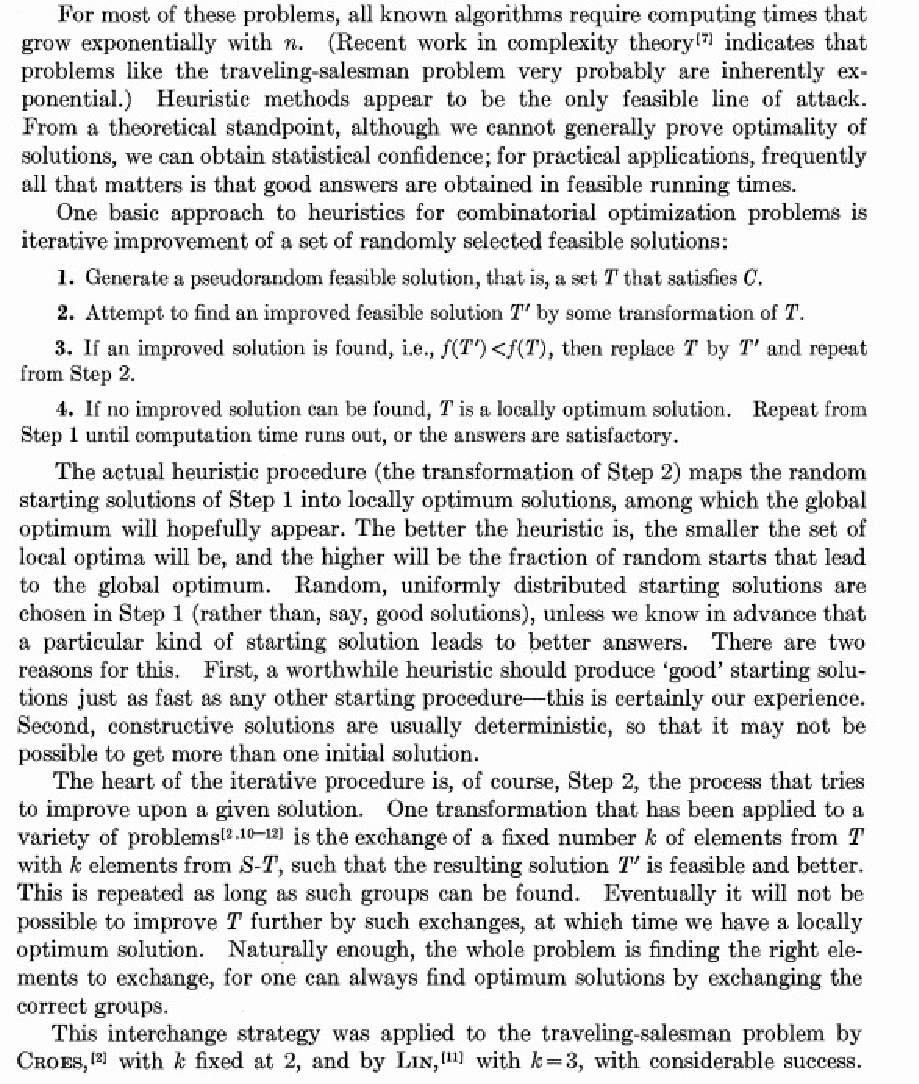
\includegraphics[width=10cm]{miscimages/linkernighan.pdf}}
  \caption{\label{fig:linkernighan} Screenshot from the Lin Kernighan paper}
\end{figure}

Page 5 of that paper contains the main sketch of the overall algorithm. 

On that note, see \cite{papadimitriou1992complexity} 
where \textit{``It is shown that finding a local optimum solution with respect
to the Lin-Kernighan heuristic for the traveling salesman problem is $PLS$-complete,''} Might have useful nuggets. 


 %\item[Approximation by Sharing] If a simple polygon $P$ on $n$ points shares $\theta n$ edges with the Delaunay 
%      Triangulation, for some constant (i.e. independent of $n$) $\theta$ close to 1 
%      are there bounds on the approximation factor (as a function of $\theta$) of how good $P$ is compared to TSP? 
\end{description}



\end{appendices}
